
\section*{Problema P8.19}

\renewcommand*\thesection{8.19}
\numberwithin{equation}{section}

\begin{center}
    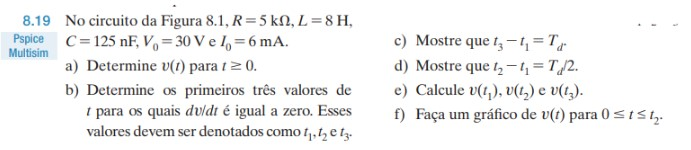
\includegraphics[scale=1.0]{P8.19.jpg}
\end{center}

\subsection*{(a)}

O primeiro passo é identificar as condições inicias de $v(t)$. Temos

\begin{equation}\label{eq:8.19.1}
    v(0) = 30 \un{V}
\end{equation}

Além disso, para a condição de inicial de $\diff{v(0)}{t}$, aplicamos análise nodal no nó superior do circuito em $t=0$, obtendo

\[ i_c(0) + i_L(0) + i_R(0) = 0  \]

\[ i_c(0) + 6 \un{mA} + \frac{v(0)}{5\un{k$\Omega$}} = 0  \]

\[ i_c(0) = - 12 \un{mA}  \]

Note que

\[ i_c = C\diff{v}{t} \logo \diff{v(0)}{t} = \frac{i_c(0)}{C} \]

Assim, subsituindo o valor de $i_c(0)$ encontrado, temos a segunda condição inicial da EDO dada por

\begin{equation}\label{eq:8.19.2}
    \diff{v(0)}{t} = -96 \un{kV/s}
\end{equation}

Como o circuito da Figura 8.1 é um circuito RLC paralelo, temos que a equação característica é dada por 

\begin{equation}\label{eq:8.19.3}
    s^2 + \frac{s}{RC} + \frac{1}{LC} = 0
\end{equation}

Que possui solução   

\[ s = \frac{-(1600) \pm \sqrt{(1600)^2 - 4(1)(10^6)}}{2(1)} \]

Note que temos o discriminante $\Delta < 0$. Nesse caso, temos soluções complexas para a equação característica e a resposta da tensão é subamortecida.

\[ s = \frac{-1600 \pm j1200}{2} \]

\[ s_1 = -800 + j600 \un{rad/s} \quad , \quad s_2 = -800 - j600 \un{rad/s} \]

Sabemos que a solução da EDO é da forma

\[ v(t) = Ae^{st}  \]

Com as duas raízes encontradas $s_1$ e $s_2$, temos que a solução geral é dada pela combinação linear

\begin{equation}\label{eq:8.19.4}
    v(t) = v_1(t) + v_2(t)
\end{equation}

Onde $v_1(t)$ e $v_2(t)$ são duas possíveis soluções para $v(t)$ dadas por  

\[ \begin{cases}
        v_1(t) = A_1e^{s_1t}  & \\
        \noalign{\vskip9pt}
        v_2(t) = A_2e^{s_2t}
    \end{cases}
\]

Diferenciando \eqref{eq:8.19.4} com respeito a $t$, temos duas equações

\[ \begin{cases}
        v(t) = A_1e^{s_1t} + A_2e^{s_2t} & \\
        \noalign{\vskip9pt}
        \diff{v(t)}{t} = A_1s_1e^{s_1t} + A_2s_2e^{s_2t}
    \end{cases}
\]

Em $t=0$, temos as condições iniciais já conhecidas em \eqref{eq:8.19.1} em \eqref{eq:8.19.2}

\[ \begin{cases}
        v(0) = A_1e^{s_10} + A_2e^{s_20} & \\
        \noalign{\vskip9pt}
        \diff{v(0)}{t} = A_1s_1e^{s_10} + A_2s_2e^{s_20}
    \end{cases}
    \logo
    \begin{cases}
        A_1 + A_2 = 30 \un{V} & \\
        \noalign{\vskip9pt}
        A_1s_1 + A_2s_2 = -96 \un{kV/s}
    \end{cases}
\]

De posse dessas equações, temos o sistema linear para identificar os coeficientes $A_1$ e $A_2$

\begingroup
\renewcommand*{\arraystretch}{1.5}

\[
    \begin{bmatrix}
        1 & 1    \\
        s_1    & s_2
    \end{bmatrix}
    \begin{bmatrix}
        A_1 \\
        A_2
    \end{bmatrix}
    =
    \begin{bmatrix}
        30 \\
        -96000
    \end{bmatrix} \logo
    \begin{bmatrix}
        -s_1 & -s_1    \\
        s_1    & s_2
    \end{bmatrix}
    \begin{bmatrix}
        A_1 \\
        A_2
    \end{bmatrix}
    =
    \begin{bmatrix}
        -30s_1 \\
        -96000
    \end{bmatrix}
\]

\[
    \begin{bmatrix}
        -s_1 & -s_1    \\
        0    & s_2 - s_1
    \end{bmatrix}
    \begin{bmatrix}
        A_1 \\
        A_2
    \end{bmatrix}
    =
    \begin{bmatrix}
        -30s_1 \\
        -96000 - 30s_1
    \end{bmatrix}
\]

\endgroup

Assim, temos  

\[ A_2 = \frac{-96000 - 30s_1}{s_2 - s_1} \logo A_2 = \frac{-96000 - 30(-800 +j600)}{-800 -j600 - (-800 +j600)}\] 

\[ A_2 = \frac{-72000 - j18000}{-j1200} \] 

\[ A_2 = 15 - j60 \quad , \quad A_1 = 15 + j60 \] 

Conhecidos coeficientes $A_1$ e $A_2$, bem como as raízes $s_1$ e $s_2$, temos a solução geral $v(t)$ na forma de \eqref{eq:8.19.4}

\[ v(t) = (15 + j60)e^{(-800 + j600)t} + (15 - j60)e^{(-800 - j600)t} \un{V} \, , \, t \geq 0  \]

Vamos remover os exponenciais complexos usando a identidade de Euler.

\[ v(t) = (15 + j60)e^{-800t}e^{j600t} + (15 - j60)e^{-800t}e^{-j600t} \]

\[ v(t) = (15 + j60)e^{-800t}(\cos(600t) + j\sin(600t)) + (15 - j60)e^{-800t}(\cos(600t) - j\sin(600t)) \]

Evidenciando o termo $e^{-800t}$ e expandindo os demais via propriedade distributiva, temos que todas 
parcelas complexas se cancelam e ficamos com

\[ \boxed{v(t) = e^{-800t}\left[30\cos(600t) - 120\sin(600t)\right] \un{V} \, , \, t \geq 0 }  \]

\subsection*{(b)}

Diferenciando $v(t)$ encontrado no item (a) com respeito a $t$, temos   

\[ \diff{v}{t} = (30\cos(600t) - 120\sin(600t))(-800)e^{-800t} + e^{-800t}(-30\sin(600t)(600) - 120\cos(600t)(600)) \]

\[ \diff{v}{t} = e^{-800t}\left[-24000\cos(600t) + 96000\sin(600t) - 18000\sin(600t) - 72000\cos(600t)\right]   \]

Para que $\diff{v}{t} = 0$, temos

\[ -24000\cos(600t) + 96000\sin(600t) - 18000\sin(600t) - 72000\cos(600t) = 0  \]

\[ \sin(600t)(96000 - 18000) - \cos(600t)(24000 + 72000) = 0  \]

\[ \frac{\sin(600t)}{\cos(600t)} = \frac{24000 + 72000}{96000 - 18000}  \]

\[ \tan(600t) = 1.23076 \logo t = \frac{\tan^{-1}(1.23076)}{600}  \]

Usando a propriedade das tangentes de 

\[ \tan(\theta) = \tan(\theta + n\pi) \, , \, n = 0, 1, 2, 3 ... \]

Temos  

\[ t = \frac{0.8884 + n\pi}{600} \, , \, n = 0, 1, 2, 3 ...  \]

Os três primeiros valores de $t$ que satisfazem são 

\[ \boxed{t_1 = 1.481 \un{ms} \, , \, t_2 = 6.717 \un{ms} \, , \, t_3 = 11.95 \un{ms}  }  \]

\subsection*{(c)}

Sabemos que frequência angular de amortecimento $\omega_d$ é dada por  

\begin{equation}\label{eq:8.19.5}
    \omega_d = \sqrt{\omega_o^2 - \alpha^2}
\end{equation}

Expandindo os termos conforme as definições,

\[ \omega_d = \sqrt{\frac{1}{LC} -  \frac{1}{4R^2C^2}} \]

O período de $\omega_d$ é 

\[ T_d = \frac{2\pi}{\sqrt{\frac{1}{LC} -  \frac{1}{4R^2C^2}} } \]

\[ T_d = 10.47 \un{ms} \]

A diferença $t_3 - t_1$ é

\[ t_3 - t_1 = 11.95 \un{ms} - 1.481 \un{ms} = 10.469 \un{ms} \]

Portanto,   

\[ \boxed{T_d = t_3 - t_1} \]

\subsection*{(d)}

Temos  

\[ \frac{T_d}{2} = \frac{10.47 \un{ms}}{2} = 5.235 \un{ms} \]

Além disso, 

\[ t_2 - t_1 = 6.717 \un{ms} - 1.481 \un{ms} = 5.236 \un{ms} \]

Portanto,  

\[ \boxed{\frac{T_d}{2} = t_2 - t_1} \]

\subsection*{(e)}

Usando o resultado do item (a), temos 

\[ v(t_1) = v(1.481 \un{ms}) = - 22.69 \un{V}   \]

\[ v(t_2) = v(6.717 \un{ms}) = - 0.344 \un{V}   \]

\[ v(t_3) = v(11.95 \un{ms}) = -5.22 \un{mV}   \]

\subsection*{(f)}

Usamos a ferramente online Desmos para plotar o gráfico de $v(t)$.

\begin{center}
    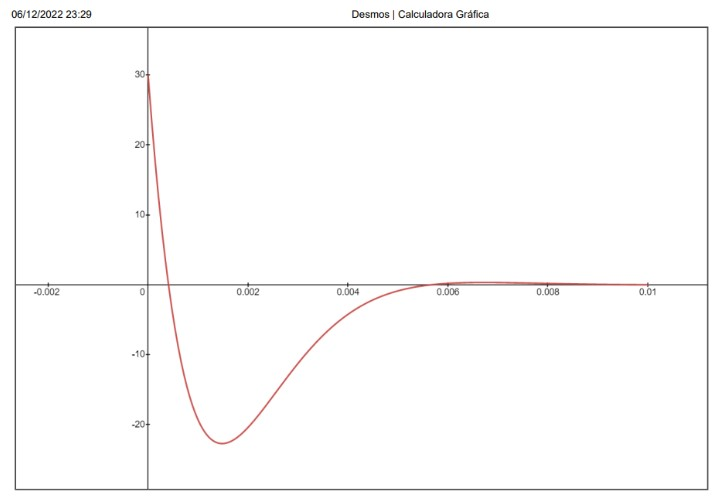
\includegraphics[scale=1.0]{P8.19-Item(f).jpg}
\end{center}

